\documentclass[11pt]{article}

\usepackage[utf8]{inputenc}
\usepackage[T1]{fontenc}

\usepackage[a4paper, left=2cm, right=2cm, top=3.5cm, bottom=3.5cm]{geometry}
\usepackage[french]{babel}

% Paragraph spacing
\setlength{\parskip}{1em}

% Fancy headers
\usepackage{fancyhdr}

% Captions for subfigures
\usepackage{subcaption}

% Code highlighting
\usepackage{minted}

% Footnote inside a caption
\usepackage{fnpos}
\usepackage{ftnxtra}

% Maths
\usepackage{amsmath}
\usepackage{amssymb}

% Todo notes
\usepackage{todonotes}

% Table of contents for bibliography
\usepackage[nottoc]{tocbibind}

% Inline monospace font
\def\code#1{\texttt{#1}}

% Figures
\usepackage{graphicx}

% Draw figures
\usepackage{tikz}

% Tikz node rotation
\usetikzlibrary{positioning}

% Turing machine
\usetikzlibrary{chains,fit,shapes}

% Usage: \rotnode[options]{rotation}{text}
\newcommand\rotnode[3][]{%
    \node [#1, opacity=0.0] (tmp) {#3};
    \node [draw, rotate around={#2:(tmp.center)}] at (tmp) {#3};
}

% Clickable links
\usepackage{hyperref}

% Table of contents depth
\setcounter{tocdepth}{2}

% Inline code
\usepackage{listings}
\usepackage{color}

\title{Systèmes d'exploitation : processus}

\author{William SCHMITT}
\date{2018-2019}

\begin{document}
\maketitle

\section{Activités parallèles}
Exemple d'activités parallèles :
\begin{itemize}
    \item Interactions avec le matériel
    \item Abstraite : logiciel, utilisateurs
\end{itemize}

\subsection{Mémoire}

Les activités parallèles sont en \textbf{compétition et en coopération} pour faire le travail demandé par l'utilisateur. Il s'agit d'écrire des programmes permettant de réaliser ces activités, en séparant les programmes par activité.
Intervient alors la notion de cohabitation entre les données et programmes différents, sachant qu'on ne dispose que d'un seul espace mémoire et un seul CPU.

La notion d'adresse virtuelle est introduite pour isoler les programmes, à l'aide d'indirections dans les adresses manipulées par les programmes. Chaque programme est isolé, permettant de garantir de la sécurité.

L'espace virtuel est coupé en pages (\textbf{pagination}).

\todo[inline]{Il manque un bout ici.}

\subsection{Processus et partage du temps}
Un millier de processus sur un système Linux, selon les paquets installés. On a donc beaucoup de processus, peu de processeurs/coeurs.
Le temps CPU est coupé en tranche de temps, les \textbf{quanta}. Initialement, le temps était géré par les processus eux-mêmes, mais en cas de boucle infinie par exemple, ils n'étaient pas capables de rendre la main.
\paragraph{Modalités de changement de processus}
\begin{itemize}
    \item Tick horloge
    \begin{enumerate}
        \item Tock horloge déclenche interruption à la fin du quantum
        \item Sauvegarde minimale (hardware, sauvegarde PC)
        \item Traitant d'interruption : sauvegarde complète (contexte du processus)
        \item Commutation de contexte : \textbf{context\_switch}
        \item Fin du traitant (du processus qui a pris la main entre temps) : restauration
        \item Retour d'interruption : restauration minimale (PC)
    \end{enumerate}
    \item I/O
    \item Terminaison de processus
    \item Synchronisation de processus
    \item sleep
\end{itemize}

\paragraph{Contexte d'un processus}
Un processus \textit{comporte} :
\begin{itemize}
    \item du code : en RAM
    \item des données \begin{itemize}
        \item en RAM
        \item dans les registres CPU : c'est ces données qui sont sauvegardées \& restaurées.
    \end{itemize}
\end{itemize}

En particulier, la sauvegarde du registre PC (instruction courante) et effectuée par le matériel.

\paragraph{Composition d'un processus}
\begin{itemize}
    \item Processus
    \begin{itemize}
        \item Espace de mémoire : virtuel et privé.
        \item 1 programme : données.
    \end{itemize}
    \item Thread (connu par l'OS): partie "exécutive" d'un processus : exécute 1 fonction.
    \item \textit{Thread users} (connu par le programme) (= fibre, task, co-routine, go-routine)
\end{itemize}

Les deux premiers points sont souvent confondus (ex. la commande ps donne le numéro de processus, mais le thread a le même numéro).

\paragraph{Ordonnanceur}
Cette fonction est appelée à chaque changement de processus et choisit le prochain processus élu parmi les processus \textbf{prêts}, on essaie de garantir la localité des informations dans le cache, selon certains critères.

Il s'agit d'optimiser le coût des interruptions (20k cycles) et de leurs traitants.

\paragraph{Etat des processus}
\begin{figure}[ht]
    \centering
    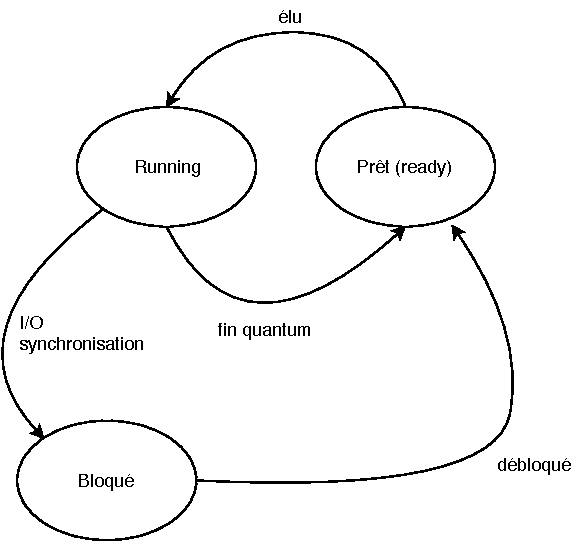
\includegraphics{img/c2-process-states.pdf}
\end{figure}

Une des structures de données fondamentales d'un système d'exploitation est une \textbf{liste} de processus dans l'état \textit{prêt}.

\todo[inline]{Il manque le morceau avec les explications sur la localité}

\subsection{Partage}

\begin{center}
    \begin{tabular}{ |c|c|c| }
        \hline
        & Processus & Thread \\
        \hline\hline
        Code & 1 & 1 fonction du code \\
        \hline
        Pile (variables locales) & Autant que de thread & 1 par thread \\
        \hline
        Fichiers (open, close, read, write) & Descripteurs de fichiers ouverts & - \\
        \hline
        Réseaux (cf. fichiers) & & \\
        \hline
        Exit (terminer un \textbf{processus}) & &\\
        \hline
        Données = variables globales (cf. code) & &\\
        \hline
    \end{tabular}
\end{center}

\section{Processus (et threads) sous UNIX}
\subsection{Outils}
\mintinline{sh}{ps}, \mintinline{sh}{htop}, \mintinline{sh}{top}, \mintinline{sh}{px}, \mintinline{sh}{pstree}

\subsection{Taille (en mémoire) d'un processus}
La taille peut faire référence à plusieurs choses :
\begin{itemize}
    \item Sa taille \textbf{complète} : si on mettait tout le processus en mémoire. La plupart des données sont inutiles.
    \item Taille en RAM : indicateur trompeur car certaines portions (comme les libs) sont partagées 
\end{itemize}
Des outils comme \mintinline{sh}{smem} partagent équitablement l'espace partagé par le nombre de processus utilisant des ressources partagées.

Lorsque le système manque de mémoire, le noyau linux appelle \mintinline{sh}{OOM_killer}, une fonction qui tue le plus gros processus (à certaines exceptions près).

\subsection{fork}
Exemple de \mintinline{c}{fork()} :
\begin{minted}{C}
    int r = fork(); // crée une copie du processus appelant
    switch(r) {
        case -1:
            perror("mon fork:");
            break;
        case 0:
            // je suis le fils
            break;
        default:
            // je suis le père de "r" (PID de mon fils)
    }
\end{minted}
Le souci de \mintinline{c}{fork()} est qu'on obtient le même processus.

\subsection{exec(p/vp/lp/e/le)}
La famille des \mintinline{c}{exec} fait du recouvrement : change le programme. L'exécution démarre donc au début du programme, mais cela ne concerne que l'exécution : les fichiers ouverts dans l'appelant sont accessibles dans l'appelé.

\subsection{wait, waitpid}
Utilisable uniquement par le père : donc un processus orphelin ne peut pas être attendu.

\subsection{Signaux}
Utilisable avec \mintinline{C}{kill(pid, signal_nr)}.
Si CTRL+C tue les processus, il laisse le temps aux processus de fermer ses fichiers, contrairement à \mintinline{sh}{kill -9}

\section{Threads}

\begin{figure}[ht]
    \centering
    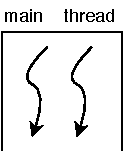
\includegraphics{img/c2-main-thread.pdf}
\end{figure}

\begin{minted}{C++}
    auto th = new thread([]( { cout <<"hello"<<endl; }));
    th->join(); // Attend la fin du thread
\end{minted}

La communication entre threads est facile (variable globale), mais l'écriture n'est pas forcément atomique.

\paragraph{Exemple :} multithread en C11 qui incrémente variable partagée par tous les threads : le résultat est bien inférieur à celui souhaité.

\subsection{Gestion de la concurrence}
Il s'agit donc de les modifier les variables d'état globales un à la fois, via (par exemple) :
\begin{itemize}
    \item Instructions atomiques : mais elles sont coûteuses et ne peuvent modifier qu'un mot à la fois.
\end{itemize}

\subsubsection{Exemple}
\paragraph{Enoncé}
Exemple de base : 2 threads exécutant \mintinline{C}{A()} et \mintinline{C}{B()} :
\begin{minted}{C}
    int a = 10;
    A() {
        a = 20;
    }
    B() {
        printf("%d\n", a);
    }
\end{minted}
\textbf{But :} afficher 20 (càd que \mintinline{C}{A()} soit finie avant que \mintinline{C}{B()} ne soit lancée)

\paragraph{Solution 1 : booléen}
\begin{minted}{C}
    bool fini = false;
    int a = 10;
    A() {
        a = 20;
        fini = true;
    }
    B() {
        while (!fini); // attente active (c'est mal !)
        printf("%d\n", a);
    }
\end{minted}
Cette stratégie ne fonctionne pas forcément : sur une architecture ARM l'ordre d'affectation des variables dans \mintinline{C}{A()} n'est pas garanti. L'attente active utilise du temps CPU, ce qui est mauvais notamment pour la batterie (fréquence au maximum pour tester une variable qui ne change pas).

\paragraph{Solution 2 : moniteurs}
Inventés par Tony Hoare, le principe des moniteurs est de faire tourner des fonctions en exclusion mutuelle. Pour gérer l'attente, Hoare introduit des \textit{variables de condition} : des files d'attente de threads avec lesquelles on peut interagir grâce à wait et signal.
\begin{minted}{C}
    mtx_t m; // un mutex
    cnd_c c;
    bool fini = false;
    int a = 10;
    A() {
        mtx_lock(&m);
        a = 20;
        fini = true;
        cnd_signal(&c);
        mtx_unlock(&m);
    }
    B() {
        mtx_lock(&m);
        while (!fini);
            cnd_wait(&c, &m); // lock automatique au réveil et unlock automatique au wait
        printf("%d\n", a);
        mtx_unlock(&m);
    }
\end{minted}

L'utilisation de \mintinline{C}{cnd_wait} permet d'éviter les cas où \mintinline{C}{B()} à la main avant \mintinline{C}{A()} et garde l'exclusion mutuelle pour exécuter son \mintinline{C}{wait()}.

\end{document}